\section{Gramáticas Independientes del Contexto}
\begin{itemize}
  \item[] Una gramática \(G = \langle V_N, V_T, P, S \rangle\) es independiente del contexto si y solo si las producciones en \(P\) son de la forma \(A\to\alpha\) con \(A \in V_N\) y \(\alpha \in (V_N \cup V_T)^*\).
  \item[] Si en particular para toda \(A\to\alpha\in P\) pasa que \(\alpha\in(V_N\cup V_T)^+\) (o sea, sin reglas borradoras), entonces decimos que \(G\) es una \textbf{gramática propia}.
\end{itemize}
\subsection{Árboles de Derivación}
Sea \(G = \langle V_N, V_T, P, S \rangle\) una gramática independiente del contexto. Un árbol de derivación de una cadena \(\omega\) en \(G\) es una estructura de árbol tal que:
\begin{itemize}
  \item Cada vértice posee una etiqueta que pertenece al conjunto \(V_N \cup V_T\cup\{\lambda\}\).
  \item La raíz del árbol posee la etiqueta \(S\).
  \item Si un vértice es interior, entonces su etiqueta pertenece al conjunto \(V_N\).
  \item Si un vértice \(v_n\) posee la etiqueta \(A\) y sus hijos \(v_1, \ldots, v_m\) poseen las etiquetas \(X_1, \ldots, X_m\), entonces \(A\to X_1\ldots X_m\in P\).
  \item Si un vértice es hoja, entonces su etiqueta pertenece al conjunto \(V_T\cup\{\lambda\}\).
  \item Si una hoja posee la etiqueta \(\lambda\), entonces es el único hijo de su.
\end{itemize}

\paragraph{Camino:} Sea \(A\in V_N\) y \(X\in V_n\cup V_T\) un vértice de un árbol de derivación. El camino de \(A\) a \(X\) es la secuencia de vértices \(A=v_1, v_2, \ldots, v_n=X\) tal que \(v_i\) es hijo de \(v_{i+1}\) para todo \(i\in\{1, \ldots, n-1\}\).

\paragraph{Altura de un árbol:} La altura de un árbol de derivación es la longitud del camino más largo de la raíz a una hoja.

\paragraph{Longitud de un camino:} La longitud de un camino es la cantidad de arcos que lo componen.

\begin{lemma}\label{lem:altura}
  Sea \(G=\langle V_N, V_T, P, S \rangle\) una gramática independiente del contexto con \(P\neq\emptyset\) y sea \(T(S)\) el árbol de derivación de \(S\) en \(G\) para algún \(\alpha\in\Sigma^*\) de altura \(h\).
  \begin{center}
    Si \(a=\max\{|\beta|: A\to\beta\in P\}\), entonces \(|\alpha|\leq a^h\)
  \end{center}
\end{lemma}

\begin{demo}[0.8\textwidth]
  Por inducción en \(h\):
  \begin{itemize}
    \item \textbf{Caso base:} \(h=0\). El único árbol de derivación posible de esta altura es el símbolo \(S\). Por lo tanto \(a^h = a ^ 0 = 1 = |S|\).
    \item \textbf{Paso inductivo:} Sea \(\mathcal{T}(S)\) el árbol de derivación para \(\alpha\) de altura \(h+1\).  Sea \(\gamma\in(V_N\cup V_T)^+\) una cadena tal que \(\gamma\Rightarrow\alpha\) en \(G\). Entonces el árbol de derivación de \(\gamma\) en \(G\) tiene altura \(h\).


  \end{itemize}
\end{demo}
\begin{demoPart}[0.8\textwidth]
  \begin{itemize}
    \item[]
      Por hipotesis inductiva, vale que \(|\gamma|\leq a^h\). Por lo tanto, \(|\alpha|\leq a^h\).

      Por otra parte, \(|\alpha|\leq a|\gamma|\) ya que en el peor de los casos cada símbolo de \(\gamma\) usa la reducción de mayor tamaño. Luego, \(|\alpha|\leq aa^h = a^{h+1}\).
  \end{itemize}
\end{demoPart}
\subsection{Gramáticas Ambiguas}
Una gramática independiente del contexto \(G\) es \textbf{ambigua} si y solo si \(\exists \alpha\in\mathcal{L}(G)\) tal que posea más de un árbol de derivación.

\paragraph{Lenguaje intrisícamente ambiguo:} Un lenguaje independiente del contexto \(L\) es \textbf{íntrisicamente ambiguo}si y solo si todas las grámaticas que lo tienen como lenguaje son ambiguas.
\paragraph{Derivación más a la izquierda:} Una \textbf{derivación más a la izquierda} \(\left(\underset{L}{\Rightarrow}\right)\) de una cadena \(\omega\) es aquella que se obtiene remplazando el primer símbolo no terminal que contenga por alguna de sus derivaciónes:
Si \(A\in V_N\), \(\alpha\in V_T^*\), \(\beta \in (V_N \cup V_T)^*\) y \(A\to\gamma\in P\) entonces \(\alpha A \beta \underset{L}{\Rightarrow}  \alpha\gamma\beta \)

\paragraph{Derivación más a la derecha:}  Una \textbf{derivación más a la derecha} \(\left(\underset{R}{\Rightarrow}\right)\) de una cadena \(\omega\) es aquella que se obtiene remplazando el último símbolo no terminal que contenga por alguna de sus derivaciónes:
Si \(A\in V_N\), \(\alpha\in (V_N \cup V_T)^*\), \(\beta \in V_T^*\) y \(A\to\gamma\in P\) entonces \(\alpha A \beta \underset{R}{\Rightarrow}  \alpha\gamma\beta \)

\subsection{Lema de Pumping para Lenguajes Independientes del Contexto}
Sea \(L\) un lenguaje independiente del contexto sobre un alfabeto \(\Sigma\), existe \(n > 0\) tal que para todo \(\alpha\in L\), \(|\alpha|\geq n\) existe \(r,x,y,z,s\in\Sigma^*\) tales que:
\begin{enumerate}
  \item \(\alpha = rxyzs\)
  \item \(|xyz|\leq n\)
  \item \(|xz| > 0\)
  \item \(\forall i\geq 0, rx^iyz^is\in L\)
\end{enumerate}
\subsubsection{Demostración}
Sea \(G=\langle V_N, V_T, P, S \rangle\) una gramática independiente del contexto y sea \(a = \max\{|\beta|: A\to\beta\in P\}\).

\begin{enumerate}
  \item Tomemos \(n = a^{|V_N|+1}\). Sea \(\alpha\in\mathcal{L}(G)\) tal que \(|\alpha|\geq n\) y sea \(T(S)\) un árbol mínimo de derivación de \(\alpha\) en \(G\), es decir tiene la mínima altura posible y tal que no existe otro con menos derivaciones.

        Por el lema \ref{lem:altura}, resulta que \(a^h\geq |\alpha|\geq n = a^{|V_N|+1}\). Por lo tanto, \(h\geq |V_N|+1\). Entonces existe algún símbolo \(b\in\alpha\) tal que su camino desde la raíz es de longitud  \(h\geq|V_N|+1\).

        Como la cantidad de símbolos no terminales es \(|V_N|\), entonces en ese camino seguramente existe un no-terminal \(A\) repetido. Recorriendo el camino de forma ascendente, buscamos sus primeras dos apariciones:

        \begin{figure}[H]
          \begin{center}
            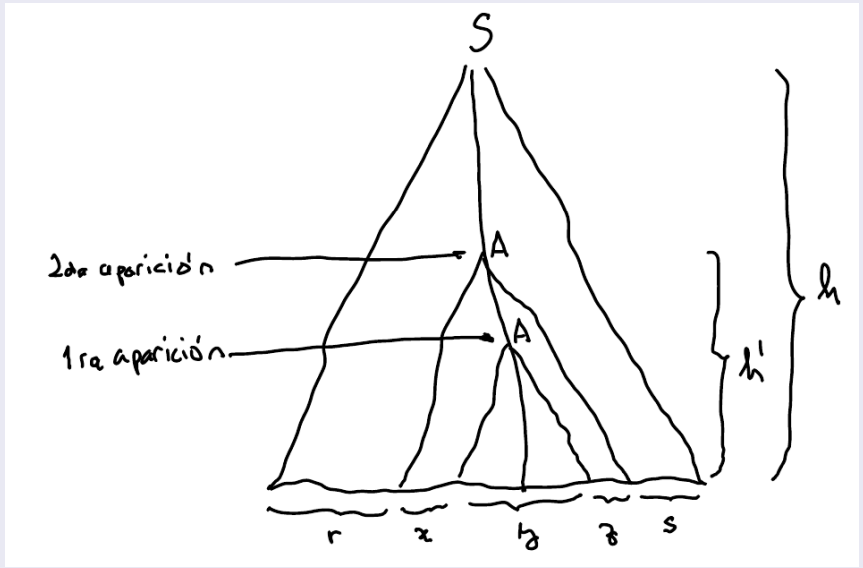
\includegraphics[scale=0.3]{imagenes/gic.pumping.tree.png}
          \end{center}
        \end{figure}

        Entonces podemos escribir \(\alpha=rxyzs\) con \(r,x,y,z\) y \(s\) como se muestra en la figura.
  \item \(|xyz|\leq n = a^{|V_n| + 1}\).
        Como \(A\) es el primer no terminal que se repite, podemos asegurar que \(h' \leq |V_N| + 1\). La segunda aparición de \(A\) tiene que pasar a lo sumo \(|V_n|\) pasos mas adelantes, sino se debería repetir otro no terminal antes. Entonces por el lema \ref{lem:altura}, resulta que \(|xyz|\leq a^{h'}\leq a^{|V_N|+1}\).
  \item \(|xz| > 0\).

        Supongamos que \(|xz| = 0\), esto quiere decir que podriamos remplazar el subárbol con raíz en la segunda aparición de \(A\) por el subárbol con raíz en la primera aparición.

        \begin{figure}[H]
          \begin{center}
            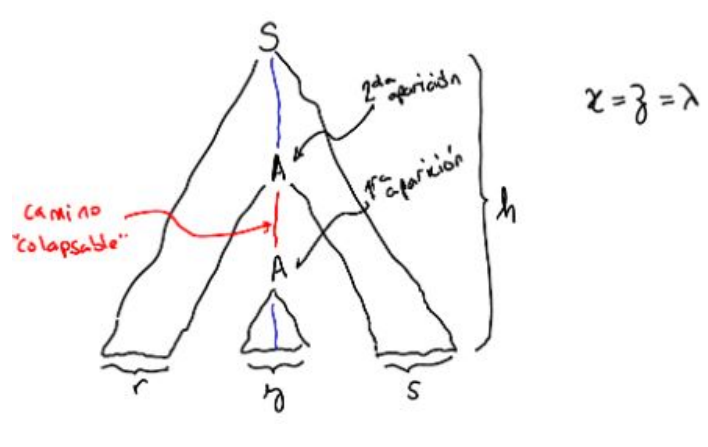
\includegraphics[scale=0.4]{imagenes/gic.pumping.tree.colapsable.png}
          \end{center}
        \end{figure}

        Esto es absurdo ya que habíamos dicho que el árbol era mínimo por lo que no debería poder colapsarse ninguno de sus caminos.

  \item \(\forall i\geq 0, rx^iyz^is\in L\)
        Finalmente, vamos a demostrar esto por inducción:
        \begin{itemize}
          \item \textbf{Caso base (\(i = 0\)):} Sabemos que \(S\deriva rAs\) y \(A\deriva y\), entonces \(S\deriva rAs\deriva rys\). Además \(rys = rx^0yz^0s\).
          \item \textbf{Paso inductivo \( i-1 \Rightarrow i\):}
                \begin{itemize}
                  \item[] \textbf{Hipotesis inductiva:} \(S\deriva rx^{i-1}Az^{i-1}s\).
                \end{itemize}
                Sabemos \(A\deriva xyz\), entonces:
                \[ S \deriva  rx^{i-1}Az^{i-1}s \Rightarrow rx^{i-1}xyzz^{i-1}s \Rightarrow rx^iyz^is \]
                Y por lo tanto \(rx^iyz^is\in L\).
        \end{itemize}
\end{enumerate}

\subsection{Propiedades de los Lenguajes Independientes del Contexto}
\begin{itemize}
  \item Si \(L_1\) y \(L_2\) son lenguajes independientes del contexto, entonces \(L_1 \cup L_2\) también lo es.
        \begin{demo}[0.8\textwidth]
          Como \(L_1\) y \(L_2\) son dos lenguajes independientes del contexto, entonces existen dos grámatica independientes del contexto \(G_1=\langle V_N, \Sigma, P_1, S_1 \rangle\) y \(G_2=\langle V_N, \Sigma, P_2, S_2 \rangle\). tales que \(L_1 = \mathcal{L}(G_1)\) y \(L_2 = \mathcal{L}(G_2)\). Supongamos, además, sin perdida de generlidad que \(V_{N_1}\cap V_{N_2} = \emptyset\). Definamos entonces:
          \[ G = \langle V_{N_1} \cup V_{N_2} \cup \{S\}, \Sigma, P_1 \cup P_2 \cup \{ S \to S_1,~S\to S_2\}, S \rangle \]

          Veamos que \(\forall\alpha\in\Sigma^*, \alpha\in\mathcal{L}(G) \iff \alpha\in\mathcal{L}(G_1) \cup \mathcal{L}(G_2)\).

          \begin{align*}
            \alpha\in\mathcal{L}(G) & \iff S\deriva\alpha \iff \red{S_1 \deriva \alpha} \lor \blue{S_2\deriva \alpha} \\
                                    & \iff \red{\alpha\in\mathcal{L}(G_1)} \lor \blue{\alpha\in\mathcal{L}(G_2)}      \\
                                    & \iff \alpha\in\mathcal{L}(G_1) \cup \mathcal{L}(G_2)
          \end{align*}
        \end{demo}
  \item Si \(L_1\) y \(L_2\) son lenguajes independientes del contexto, entonces \(L_1L_2\) también lo es.
        \begin{demo}[0.8\textwidth]
          Como \(L_1\) y \(L_2\) son dos lenguajes independientes del contexto, entonces existen dos gramáticas independientes de contexto \(G_1=\langle V_{N_1}, \Sigma, P_1, S_1 \rangle\) y \(G_2=\langle V_{N_2}, \Sigma, P_2, S_2 \rangle\) tales que \(L_1 = \mathcal{L}(G_1)\) y \(L_2 = \mathcal{L}(G_2)\). Supongamos, además, sin perdida de generlidad que \(V_{N_1}\cap V_{N_2} = \emptyset\). Definamos entonces:
        \end{demo}
        \begin{demoPart}[0.8\textwidth]
          \[ G = \langle V_{N_1} \cup V_{N_2} \cup \{S\}, \Sigma, P_1 \cup P_2 \cup \{ S \to S_1S_2\}, S \rangle \]

          Veamos que \(\forall\alpha\in\Sigma^*, \alpha\in\mathcal{L}(G) \iff \alpha\in\mathcal{L}(G_1)\mathcal{L}(G_2)\).

          \begin{align*}
            \alpha\in\mathcal{L}(G) & \iff S\deriva\alpha \iff S_1S_2\deriva\alpha                                                                            \\
                                    & \iff\exists\beta_1,\beta_2\in\Sigma^*:~\alpha=\beta_1\beta_2\land \red{S_1\deriva\beta_1}\land \blue{S_2\deriva\beta_2} \\
                                    & \iff\red{\beta_1\in\mathcal{L}(G_1)} \land \blue{\beta_2\in\mathcal{L}(G_2)}                                            \\
                                    & \iff \beta_1\beta_2 = \alpha\in\mathcal{L}(G_1)\mathcal{L}(G_2)                                                         \\
          \end{align*}
        \end{demoPart}
  \item Si \(L\) es un lenguaje independiente del contexto, entonces \(L^+\) también lo es.
        \begin{demo}[0.8\textwidth]
          Como \(L\) es un lenguaje independiente del contexto, entonces existe una gramática independiente del contexto \(G=\langle V_N, \Sigma, P, S \rangle\) tal que \(L = \mathcal{L}(G)\). Definamos entonces:

          \[ G^+ = \langle V_N \cup \{S\}, \Sigma, P \cup \{ S' \to SS',~S'\to S\}, S'\rangle \]

          Veamos que \(\mathcal{L}(G') = L^+ \)

          \begin{align*}
            \alpha\in\mathcal{L}(G') & \iff S'\deriva\alpha \iff \red{SS' \deriva \alpha}\lor\blue{S\deriva\alpha}
          \end{align*}

          Supongamos que \(\blue{S\deriva\alpha}\), entonces trivialmente vale \(\alpha\in L\subseteq L^+\).

          Por inducción, Supongamos que \(S' \deriva\beta\in L^+\): Sea \(\alpha =\gamma\beta\) con \(\gamma\in\Sigma^*\). Entonces \(SS'\deriva\alpha \iff SS'\deriva\gamma\beta \iff S\deriva\gamma \land S'\deriva\beta\)
          Entonces pasa que \(\gamma\in L\) y, por hipotesis inducción,\(\beta\in L^+\), Luego \(\gamma\beta\in L^+\)
        \end{demo}
  \item  Si \(L\) es un lenguaje independiente del contexto, entonces \(L^*\) también lo es.
        \begin{demo}[0.8\textwidth]
          Como \(L\) es un lenguaje independiente del contexto, entonces existe una gramática independiente del contexto \(G=\langle V_N, \Sigma, P, S \rangle\) tal que \(L = \mathcal{L}(G)\). Definamos entonces:
          \[
            G^* = \langle V_N \cup \{S\}, \Sigma, P \cup \{ S' \to SS',~S'\to \varepsilon\}, S'\rangle
          \]

          Veamos que \(\mathcal{L}(G^*) = L^*\). Esta demonstración es símilar a la anterior. La única defirencia es que en algún momento, en vez de usarse la regla \(S'\to S\), se usa la regla \(S'\to \varepsilon\).
        \end{demo}
  \item Si \(L_1\) y \(L_2\) son lenguajes independientes del contexto, entonces \(L_1\cap L_2\) no siempre es lenguaje independiente del contexto.
        \begin{demo}[0.8\textwidth]
          Sean \(L_1 = \{ a^n b^m c^l: n,m,l \geq 0 \land n = m \}\) y \(L_2 = \{ a^n b^m c^l : n \geq 0 \land m = l \}\) dos lenguajes independientes de contexto (\red{Demostrar?}).
          Pero \(L_1\cap L_2 = \{ a^n b^m c^l : n,m,l \geq 0 \land n = m = l \}\) no es lenguaje independiente como puede demostrarse utilizando el lema de pumping.
        \end{demo}
  \item El lenguaje \(L = \{ ww : w \in \Sigma^* \}\) no es independiente del contexto.
        \begin{demo}[0.8\textwidth]
          Sea \(L_1 = \{ a^n b^m a^n b^m:~ n,m\geq 0\}\) es tal que \(L_1 = L \cap a^* b^* a^* b^*\)
          donde \(a^* b^* a^* b^*\) es un lenguaje regular.

          La interesección entre un lenguaje regular y un lenguaje independiente de contexto da como resultado  un lenguaje independiente de contexto (\red{Demostrar?}).

          Entonces, si \(L\) fuera independiente del contexto, \(L_1\) tambien debiera serlo. Veamos que \(L_1\) no es independiente de contexto:

          Analizemos las componsiciones disponibleas para la cadena \(a^n b^n a^n b^n \in L_1\):
          \begin{figure}[H]
            \begin{center}
              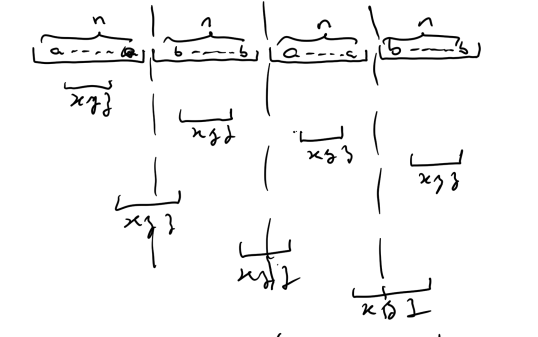
\includegraphics[scale=0.3]{imagenes/anbnanbn.png}
            \end{center}
          \end{figure}
          En los primeros cuatro casos se desbalancean la cantidad de \(a\) o \(b\), respectivamente y en el último caso se desbalancean la cantidad de \(a\) y \(b\) simultaneamente.
        \end{demo}
\end{itemize}

\subsubsection{Lenguajes libres de contexto deterministicos}
Un lenguaje \(L\) es libre de contexto deterministicos si existe un autómata de pila determinista \(A\) tal que \(L = \mathcal{L}(A)\).

Para ver más sobre lenguajes libres de contexto deterministicos, ver \href{https://www.cubawiki.com.ar/images/f/ff/TLeng_Resumen_Final_2022.pdf}{Wikipedia}.
\begin{lemma}
  El conjunto de lenguajes libres de contexto deterministicos es cerrado por la complementación.
\end{lemma}

\begin{teorema}
  Para todo automáta de pila \(M\), existe otro automáta de pila \(M'\) equivalente que siempre consume toda la cadena de entrada.
\end{teorema}
\begin{teorema}
  El complemento de un lenguaje independiente del contexto deterministico es un lenguaje independiente del contexto deterministico.
\end{teorema}
\begin{teorema}
  Existe un lenguaje independiente del contexto que es \textbf{no-deterministíco}
\end{teorema}
\begin{demo}[0.8\textwidth]
  Consideremos el lenguaje \(L = a^k b^k c^k, k\geq 0\). Sabemos que \(L\) no es independiente del contexto. Su complemento puede escribirse como:
  \begin{align*}
    \bar{L}= \{ a^i b^j c^k : i,j,k \geq 0 \land i \neq j \} \cup \{ a^i b^j c^k : i,j,k \geq 0 \land j \neq k \} \cup \overline{a^* b^* c^*}
  \end{align*}

  Osea que \(\overline{L}\) puede escribirse como la unión de dos lenguajes independientes del contexto y un lenguaje regular. Es, por lo tanto, independiente del contexto.

  Supongamosq que \(\overline{L}\) es un lenguaje independiente del contexto deterministico. Entonces, \(\overline{\overline{L}}\) también debería serlo por el teorema anterior. Pero \(\overline{\overline{L}} = L\) que ni siquiera es un lenguaje independiente del contexto. Luego \(\overline{L}\) no es deterministico.
\end{demo}

\subsection{Gramáticas propias}
\subsubsection{Conjunto de símbolos activos}
\paragraph{Símbolo alcanzable:} Dada una grámatica \(G=\langle V_N, V_T, P, S\rangle\), un símbolo \(A\in V_N\) es alcanzable si existe una forma sentencial que lo contiene,  \(S\deriva \dots A\dots\).

\paragraph{Símbolo activo:} Dada una grámatica \(G =\langle V_N, V_T, P, S\rangle\) un símbolo \(A\in V_N\) es activo si existe \(\alpha\in V_T^*\) tal que \(A\deriva \alpha\).

\paragraph{Símbolo útil:} Un no terminal \(A\) es útil si y solo si es parte de una forma sentencial que genera una cadena de terminales, osea, si \(S\deriva \alpha A\beta \deriva \omega\) con \(\omega \in \Sigma^*\) y \(\alpha, \beta \in (V_T\cup V_N)^*\).

\paragraph{Algoritmos para conseguir el conjunto de no-terminales activos de una gramática:}
\begin{algorithmic}
  \Function{activos}{\(\langle V_N, V_T, P, S\rangle\): Gramática}
  \State \(\texttt{Act}\gets\emptyset\)
  \Repeat
  \For{\(A\to \alpha \in P\)}
  \If{\(\alpha \in (\texttt{A}\cup V_T)^*\)}
  \State\(\texttt{Act}\leftarrow\texttt{Act}\cup \{A\}\)
  \EndIf
  \EndFor
  \Until{ \texttt{Act} no cambie}
  \State \Return \texttt{Act}
  \EndFunction
\end{algorithmic}

\subsubsection{Conjunto de símbolos anulables}
\begin{lemma}
  Sea G una gramática libre de contexto. Entonces existe una grámatica propia (sin producciones borradoras) \(G'\) tal que genere el mismo lenguaje que G sin la cadena nula.
\end{lemma}

\paragraph{No terminal anulable:} Un no terminal \(A\) es anulable si y solo  \(A\deriva \varepsilon\).

\paragraph{Algoritmo para conseguir el conjunto de no terminales anulables de una gramática:}

\begin{algorithmic}
  \Function{anulables}{\(\langle V_N, V_T, P, S\rangle\): Gramática}
  \State \(\texttt{An}\gets\emptyset\)
  \For{\(A\to \alpha \in P\)}
  \If{\(\alpha = \lambda\)}
  \State\(\texttt{An}\leftarrow\texttt{An}\cup \{A\}\)
  \EndIf
  \EndFor
  \Repeat
  \For{\(A\to \alpha \in P\)}
  \If{\(\alpha \in \texttt{An}^*\)}
  \State\(\texttt{An}\leftarrow\texttt{An}\cup \{A\}\)
  \EndIf
  \EndFor
  \Until{ \texttt{An} no cambie}
  \State \Return \texttt{Anul}
  \EndFunction
\end{algorithmic}

\subsubsection{Gramáticas reducidas}
\paragraph{Grámatica reducida:} Una gramática \(G = \langle V_N, V_T, P, S\rangle\) es reducida si y solo si para todo \(A\in V_N\) se cumple que \(A\) es alcanzable y activo.
\paragraph{Algoritmo para conseguir una gramática propia:}

\begin{algorithmic}
  \Function{propia}{\(G=\langle V_N, V_T, P, S\rangle\): Gramática}
  \State \(\texttt{An}\gets\texttt{anulables}(G)\)
  \For{\(A\to \alpha \in P\)}
  \If{\(\alpha = X_1\dots X_k\) con \(X_{j_1}, \dots, X_{j_m} \in \texttt{An}\)}
  \State Agregar todas las producciones \(A\to\alpha'\) donde las \(\alpha'\) se obtiene eliminando cada subconjunto en \(X_{j_1}, \dots, X_{j_m}\) de \(\alpha\). Si todos los símbolos de \(\alpha\) son anulables, no agregar \(A\to \lambda\).
  \EndIf
  \If{\(\alpha = \lambda\)}
  \State Eliminar la producción \(A\to \lambda\)
  \EndIf
  \EndFor
  \State \Return G modificada
  \EndFunction
\end{algorithmic}

\subsubsection{Forma normal de Chomsky}
Una gramática \(G = \langle V_N, V_T, P, S\rangle\) está en forma normal de Chomsky si y solo si todas sus producciones son de la forma \(A\to BC\) o \(A\to a\), donde \(A, B, C \in V_N\) y \(a \in V_T\).

Si \(L\) un lenguaje independiente del contexto tal que \(\lambda\notin L\) entonces existe una gramática \(G\) en forma normal de Chomsky.

\subsubsection{Forma normal de Greibach}
Una gramática \(G = \langle V_N, V_T, P, S\rangle\) está en forma normal de Greibach si y solo si todas sus producciones son de la forma \(A\to a\alpha\) donde \(A\in V_N\), \(a\in V_T\) y \(\alpha \in V_N^*\).

Si \(L\) un lenguaje independiente del contexto tal que \(\lambda\notin L\) entonces existe una gramática \(G\) en forma normal de Greibach.

\subsection{Otras propiedades}
\begin{itemize}
  \item Si \(M = \langle Q, \Sigma, \delta, q_0, Z_0, F\rangle\) es un autómata de pila y \(L\) el lenguaje tal que \(L = \mathcal{L}_\lambda(M)\), entonces \(L\) es independiente del contexto.
  \item Sea \(G = \langle V_N, V_T, P, S\rangle\) una grámatica independiente del contexto. Se puede construir un autómata de pila  M tal que \(\mathcal{L}(G) = \mathcal{L}_\lambda(M)\).
\end{itemize}